\documentclass{article}[12pt]
\usepackage[top=1in,bottom=1in,right=1in,left=1in]{geometry}
\usepackage{graphicx}
\usepackage{caption}
\usepackage{subcaption}
\usepackage{amsmath}
\usepackage{placeins}
\usepackage{csvsimple}
\usepackage{hyperref}
\usepackage{mathptmx}
\usepackage{times} 
\usepackage{xcolor}
%\usepackage{subfigure}
\usepackage{comment}
\graphicspath{ {./Data/} }

\begin{document}


\title{Homework Assignment 11}
\date{May 4, 2022}

\author{
  Marium Yousuf\\
  myousuf@email.arizona.edu\\
  Kayla Bennett \\
  mbennett3@email.arizona.edu
}

\maketitle
\noindent

\section{Introduction}

In this assigment we implemented the RANSAC algorithm to fit a line, solidified understanding of planar homography, and explored multi-view geometric constraints for keypoint matching. We also looked at the configuration of a fundamental matrix and image stitching using SIFT, homography, and RANSAC.

\subsection{Contributions}
Kayla contributed with SIFT extractions, arranging SIFT features, and SIFT visualizations. Marium implemented RANSAC algorithm, the Direct Linear Transform method to compute homography between two planar images, and used the homography with RANSAC to improve keypoint matching. Both discussed the derivation of fundamental matrix and image stitching and Marium was primarly responsible for implementing them. Both also consulted each other back and forth when either was stuck. 
\section{A: RANSAC}
For this part, we used a dataset of $(x, y)$ coordinates to fit a line model using a RANSAC algorithm. As provided, at least $1/4$th of the points were assumed to be close to the good fit. Fig.~\ref{fig:line} shows the scatter plot of the data points together with the line fit found with an error of 0.0928. The RANSAC algorithm was implemented as follows:
\begin{itemize}
	\item we computed $k$, the number of iterations, using the formula $\left \lceil \frac{\log (1 - p)}{\log (1 - w^n)} \right \rceil$, where $p$ quantifies the probability of success we require from the algorithm, $w$ is the probability of getting an inlier, and $n$ is the number of points needed to fit the model. We set $p = 0.99$, that is we required the algorithm to compute with 99\% success rate, $w = 0.6$, that is we wanted the inlier points ratio to be $3/5$ of the data points around the line that fit the model, and $n = 2$ since we only need 2 points to fit a line. This computed the value for our $k=11$ as the number of iterations. 
	\item using the $k$ found, we excluded picked two random points from the dataset and used the homogenous least squares model to find a line instance. For each of these instances, we computed a perpendicular distance for each of the points using a threshold of $0.2$. That is, if for any point the distance was within $0.2$ of the line distance, we included that point as an inlier. The value for the threshold was chosen by consulting the scatter plot of the data points.
	\item if the amount of inliers found exceeded 75 ($1/4$th of our 300 data points), then we assume to have found a good model and fit a line using all the inliers and the two randomly sampled points. The red line shown in Fig.~\ref{fig:line} is this line model.
\end{itemize} 

\begin{figure}[ht]
	\center
	{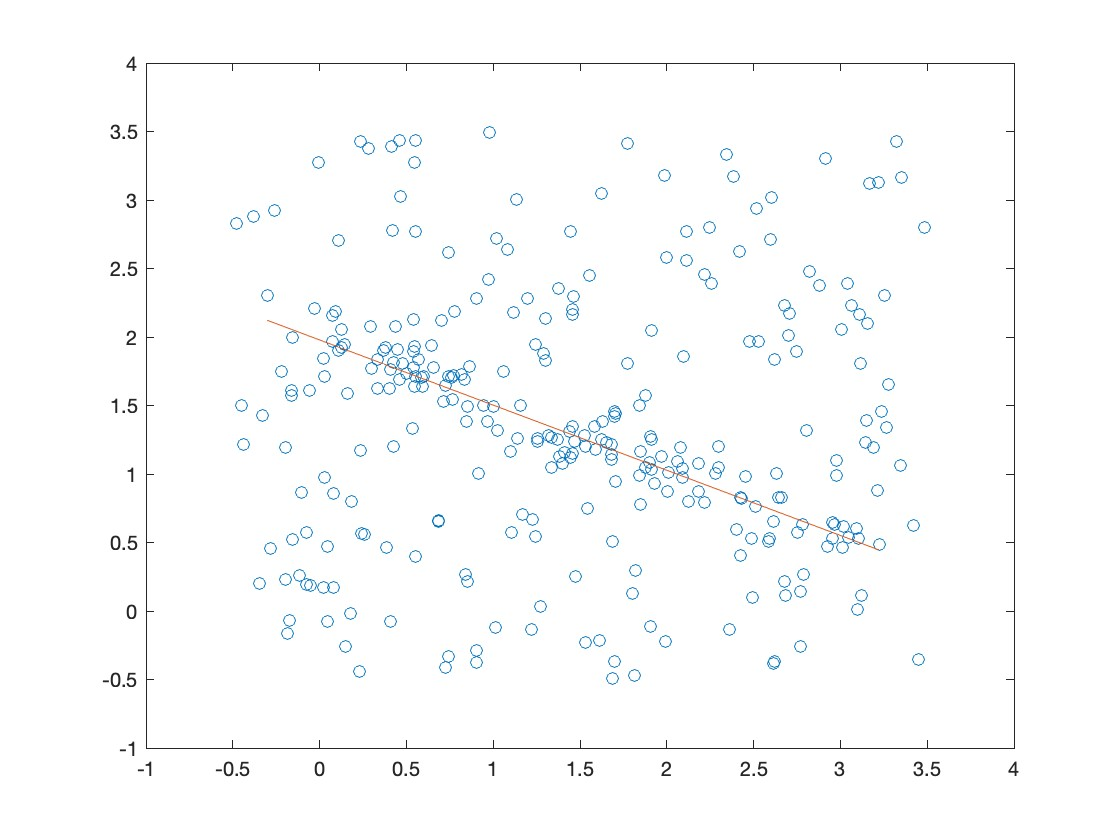
\includegraphics[width=5in]{figs/ransac_fit.jpg}}
    \caption{Figure showing the data points of $(x, y)$ coordinates as a scatter plot and a line model fitted using the RANSAC algorithm. This line was found with an error of 0.0928 based on inliers found from the algorithm.}
    \label{fig:line}
\end{figure} 
\clearpage
\section{B: Homography}
For this part, we implemented the Direct Linear Transform (DLT) method and tested it on the synthetic data and the slide/frame image pair data from assignment 9. For the synthetic data, we randomly generated 4, 5, and 6 pairs of $(x, y)$ coordinates, twice: one as "actual" points and one as the "estimate" or the point match. We did this $10$ times and yield the RMS errors as shown in Table~\ref{table:rms} below. It's a little difficult to tell if the code is working since the errors stay between (0.3, 0.4) (range tested through trial-and-error) for any number of pairs. We conclude that since we only need 4 good matches, the number of pairs is not making much of a difference in the homography found using the DLT method.

\begin{table}[h]
\begin{center}
\begin{tabular}{|c|c|c|c|c|}
\hline
Number of Pairs & RMS  \\
\hline
4 & 0.3108 \\
\hline
5 & 0.3235 \\
\hline
6 & 0.3267 \\ 
\hline
\end{tabular}
\end{center}
\caption{ RMS error of the transformation for 4, 5, and 6 randomly generated pairs of $(x, y)$-coordinates lying between a $[0,1]\times[0,1]$ window.}
\label{table:rms}
\end{table}

Moving on to the slide/frame image pairs, we collected 8 distinct points using mouse clicks as shown in Fig.~\ref{fig:slideframe} for all three slide/frame pairs. Then using 4 of these clicked points, we computed the homography using the DLT method for each slide/frame pair. Using this homography, we estimated the corresponding slide coordinates to the points on the video frame image. The Fig.~\ref{fig:slideframe_est} shows the visualization on the video frame images, displaying the 8 clicked points in red and the 8 mapped locations in yellow. {\it Please note: previously, we had issue with DLT due to which the estimated (yellow) points were shifted. This issue occured because of two things: 1) we were rescaling the points to [0, 1], and 2) we forgot to normalize the homogenous coordinates so that the last column had all 1s.}

\clearpage
\begin{figure}[ht]
	\begin{subfigure}{0.5\textwidth}
	    {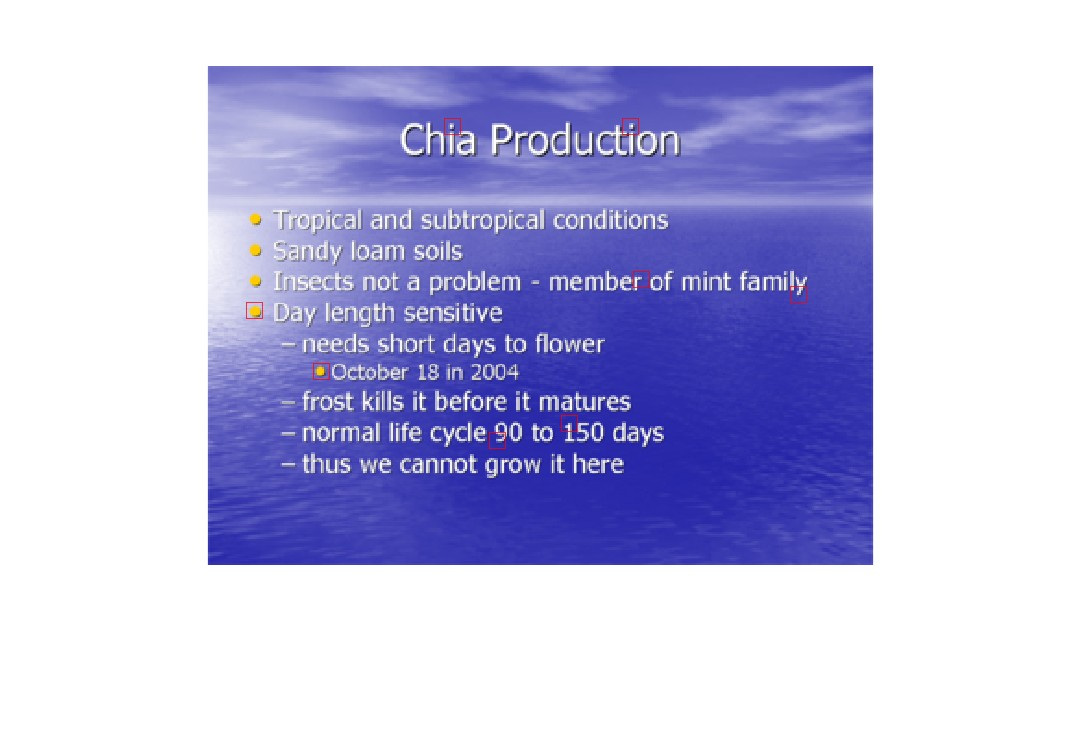
\includegraphics[width=3in]{figs/vizSlidePts_1.jpg}}
		\caption{Slide 1}
	\end{subfigure}
	\begin{subfigure}{0.5\textwidth}
	    {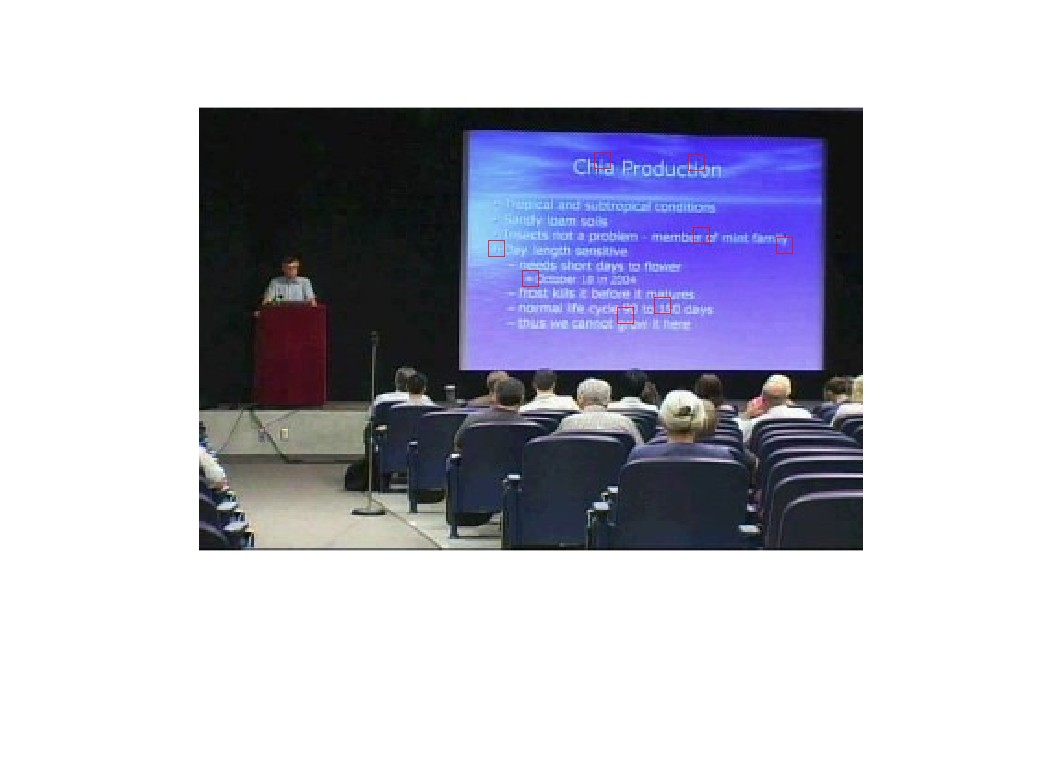
\includegraphics[width=3in]{figs/vizFramePts_1.jpg}}
		\caption{Frame 1}
	\end{subfigure}
	\begin{subfigure}{0.5\textwidth}
	    {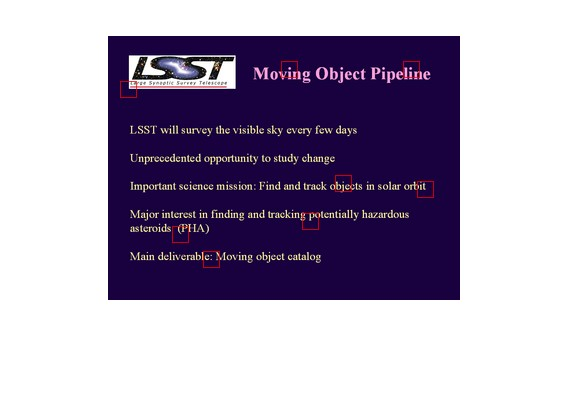
\includegraphics[width=3in]{figs/vizSlidePts_2.jpg}}
		\caption{Slide 2}
	\end{subfigure}
	\begin{subfigure}{0.5\textwidth}
	    {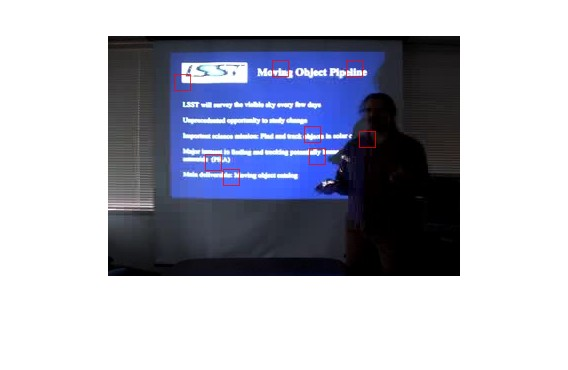
\includegraphics[width=3in]{figs/vizFramePts_2.jpg}}
		\caption{Frame 2}
	\end{subfigure}
	\begin{subfigure}{0.5\textwidth}
	    {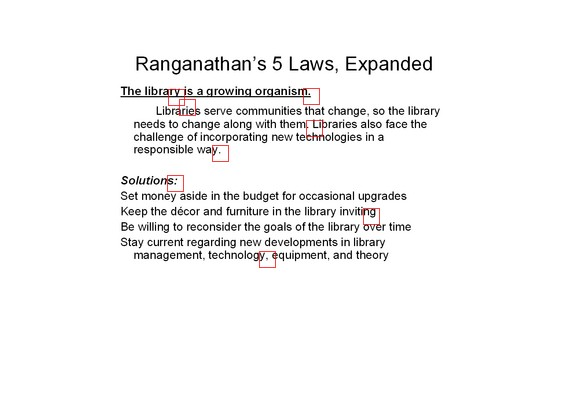
\includegraphics[width=3in]{figs/vizSlidePts_3.jpg}}
		\caption{Slide 3}
	\end{subfigure}
	\begin{subfigure}{0.5\textwidth}
	    {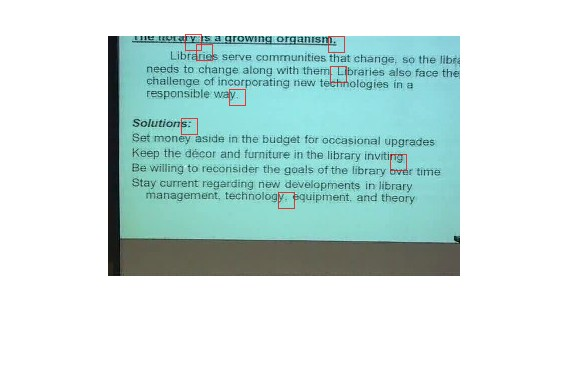
\includegraphics[width=3in]{figs/vizFramePts_3.jpg}}
	    \caption{Frame 3}
	\end{subfigure}
	\caption{Figure showing collected 8 matching points using manual mouse clicking. The points were chosen by focusing on distinct locations that were least ambiguous.}
	\label{fig:slideframe}
\end{figure}

\clearpage
\begin{figure}[ht]
	\begin{subfigure}{0.4\textwidth}
	    {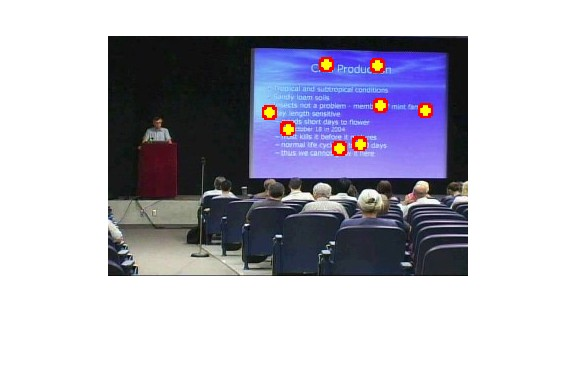
\includegraphics[width=3in]{new_figs/fBSF1.jpg}}
		\caption{Estimated points for Frame 1}
	\end{subfigure}
	\begin{subfigure}{0.4\textwidth}
	    {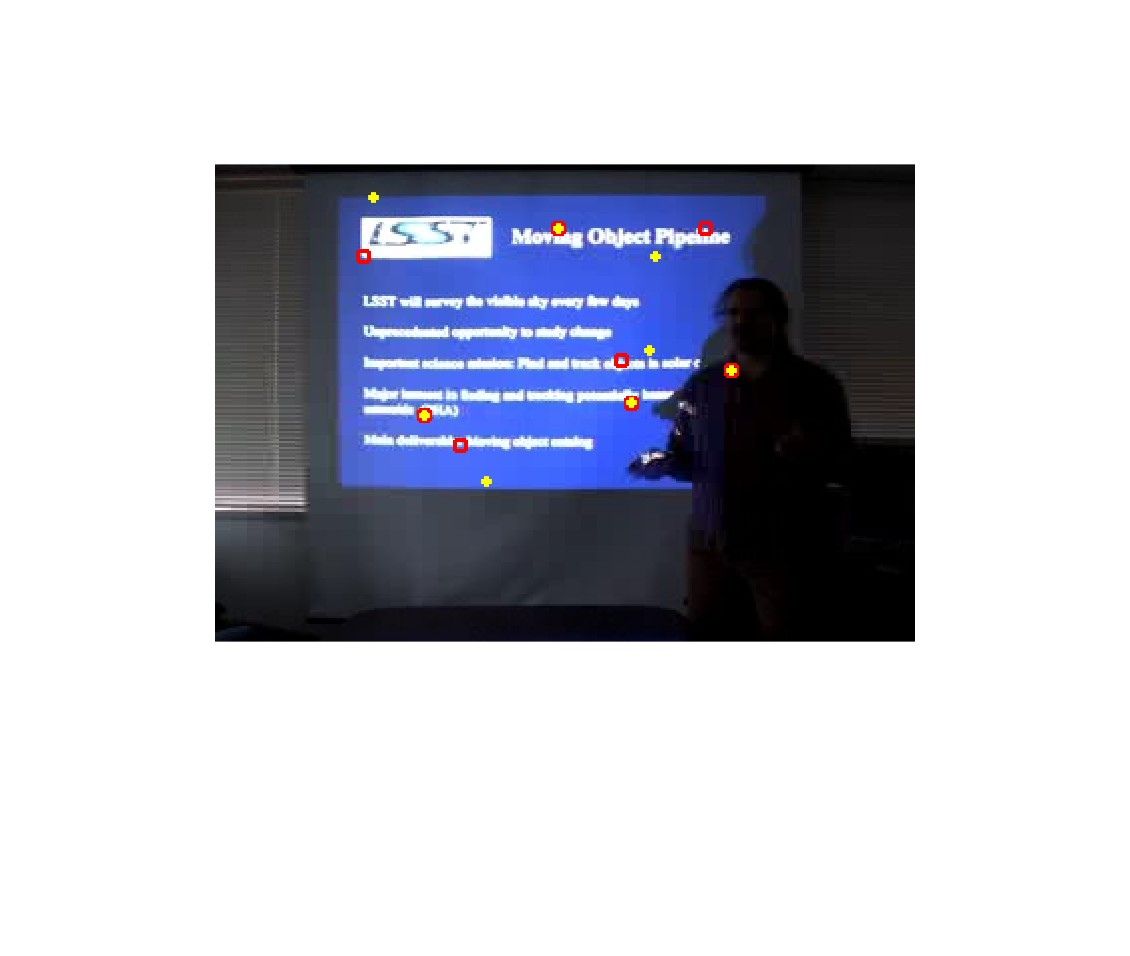
\includegraphics[width=3in]{new_figs/fBSF2.jpg}}
		\caption{Estimated points for Frame 2}
	\end{subfigure}
	\begin{subfigure}{0.4\textwidth}
	    {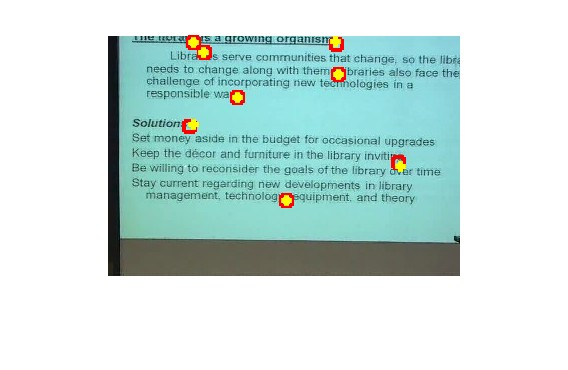
\includegraphics[width=3in]{new_figs/fBSF3.jpg}}
		\caption{Estimated points for Frame 3}
	\end{subfigure}
	\caption{Figure showing the clicked points (in red) against the estimated points computed using homography (in yellow). Note that the subset of points chosen to compute the homography have a visible overlap (that is, yellow marker is perfectly contained in the red square).}
	\label{fig:slideframe_est}
\end{figure}

% RMS errors yielded for each pair are shown in Table~\ref{table:rmssf}
% \begin{table}[h]
% \begin{center}
% \begin{tabular}{|c|c|c|c|c|}
% \hline
% Slide/Frame Pair & RMS  \\
% \hline
% Slide/Frame 1 & 0.1750 \\
% \hline
% Slide/Frame 2 & 0.1756 \\
% \hline
% Slide/Frame 3 & 0.1947 \\ 
% \hline
% \end{tabular}
% \end{center}
% \caption{ RMS error of the difference between the clicked points and the estimated points on the video frame images.}
% \label{table:rmssf}
% \end{table}


\clearpage
\section{C: Homography and RANSAC}
For this part we again used the slide/frame image pairs from assignment 9 to compute homography for several points (instead of the mouse-clicks chosen in Part B) using the RANSAC algorithm. We achieved some meaningful results by doing the following: 

\begin{itemize}
	\item for each slide/frame pair, we used the {\it .sift} files from assignment 9 for SIFT features and created a $M \times 11$ matrix holding the $(x, y)$ coordinates, scale, and direction for video frame image, corresponding $(x, y)$ coordinates, scale, and direction for the slide image, their corresponding Euclidean distance using the nearest neighbor between their 128-element feature vector, angles between their corresponding 128-element feature vector, and Chi-squared measure between their 128-element feature vector. $M$ is the number of features extracted returned by the SIFT. 
	\item we sorted our data matrix by the Euclidean distance and used it as our data set for the RANSAC algorithm, which we ran $k = 178$ times, computed with $n=4$ (number of data points for the model -- need 4 for homography), $w = 0.4$ (the inlier ratio), and $p=0.99$ (the success probability).
	\item for each slide/pair image, we found the best homography $H$, using 4 random rows from the matrix as our inliers, their DLT as our initial model, and then used the frame keypoints from the rest of the data to estimate the slide keypoints. If the RMS between the slide coordinates from the original data matrix and the estimated slide keypoints was within a threshold (chosen as 50), then we included that estimate in our inlier set. 
	\item once the size of the inlier set was over some set value (of $N=150)$, we assumed to have found a good model and recomputed our homography using the DLT with the intial inliers and additional inliers that hold the threshold. 
	\item Fig.~\ref{fig:slideframeC} shows the mapping of keypoints from estimated slide image to the corresponding keypoints on the video frame.  
\end{itemize}

Challenges faced: initally, we had major trouble trying to match the keypoints to reasonable estimated keypoints (going both slide to frame and frame to slide). The estimated keypoints seemed to be in the vicinity of where they should land and by close observation the line often crossed where it supposedly should be... it also looked like the estimated points are bunching up together. After some time-consuming debugging, it turned out there were a couple issues: the RANSAC threshold to decide on the inliers needed reconfiguration and although we were normalizing the estimated keypoints so that the last column of homogenous coordinates was always full of 1s, we were doing it in one line of code and we just had to split them into multiple lines to get the desired results. 

% e double checked and it was not the issue of the visualization, but we also couldn't figure out what's going awry. From the results of Part B), it seems the DLT is working correctly. We also tried decreasing the inlier ratio to increase the number of iterations $k$ for the RANSAC algorithm, but got similar results as shown in Fig.~\ref{fig:slideframeC}. 

\begin{figure}[ht]
	\begin{subfigure}{0.4\textwidth}
	    {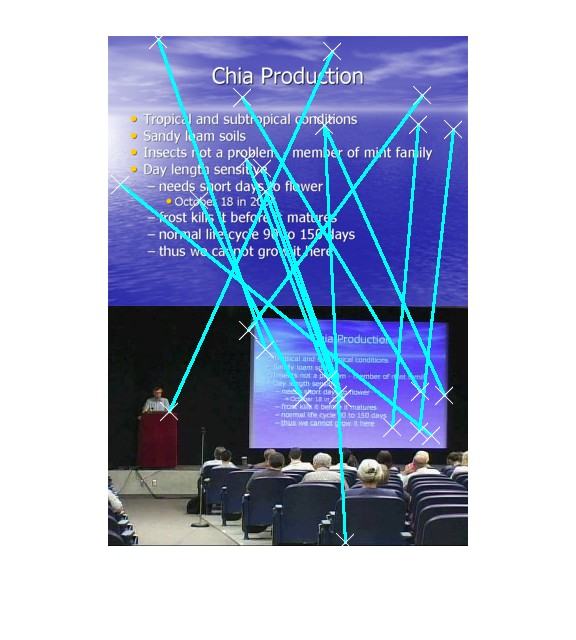
\includegraphics[width=3in]{new_figs/fCSF1x.jpg}}
		\caption{Slide/Frame 1 - First pair seems to perform the worst; on close inspection, the gradient (going from purplish tone to blue) on the slide is opposite to gradient on the frame. Therefore, multiple keypoints are matched opposite considering the water-like texture/background of the slide/frame.}
	\end{subfigure}
	\begin{subfigure}{0.4\textwidth}
	    {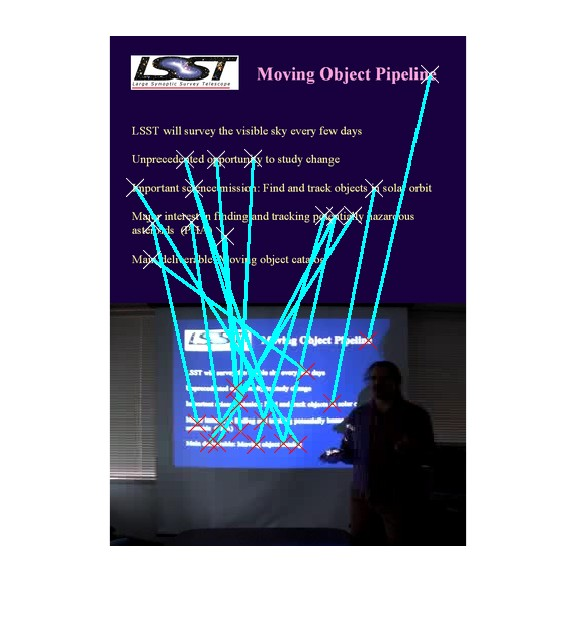
\includegraphics[width=3in]{new_figs/fCSF2x.jpg}}
		\caption{Slide/Frame 2 - Second pair performed better than the first. There are still some mis-matches, but we were happy to see the perfect matches like the end of word "pipeline", "in" in the third line, and so on.}
	\end{subfigure}
	\begin{subfigure}{0.4\textwidth}
	    {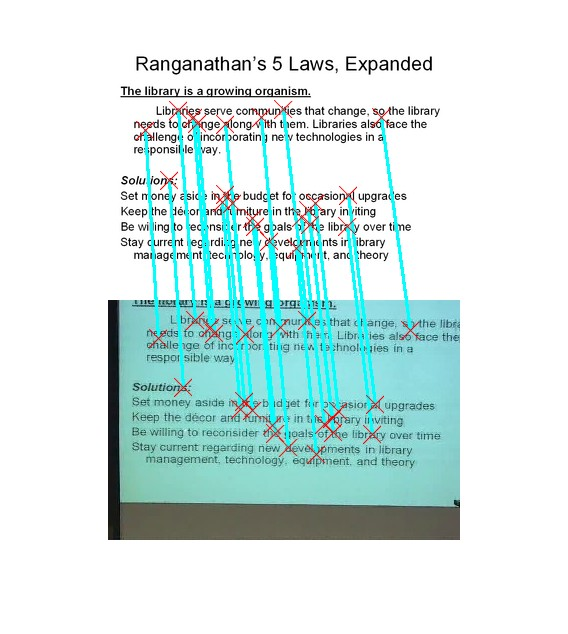
\includegraphics[width=3in]{new_figs/fCSF3x.jpg}}
	    \caption{Slide/Frame 3 -  Third pair performed the best.}
	\end{subfigure}
	\caption{ Figure showing the mapping of keypoints for the provided slide-frame pairs. These slide keypoints were estimated from the frame keypoints using the homography computed with RANSAC algorithm. We picked our keypoints based on the lowest Euclidean distance and were getting similar results using the distance between the matches as the angle between feature vectors.}
\label{fig:slideframeC}
\end{figure}

\clearpage
\section{D1: Configuring a fundamental matrix}
\subsection{} 

Fig.~\ref{fig:fmkeypoints} shows the 20 matching image points using mouse-clicking as done in HW3 previously. These coordinates were saved and submitted with the submitted assignment files named {\it FM\_1.txt} and {\it FM\_2.txt}. 

\begin{figure}[ht]
\centering
	\begin{subfigure}{0.5\textwidth}
    {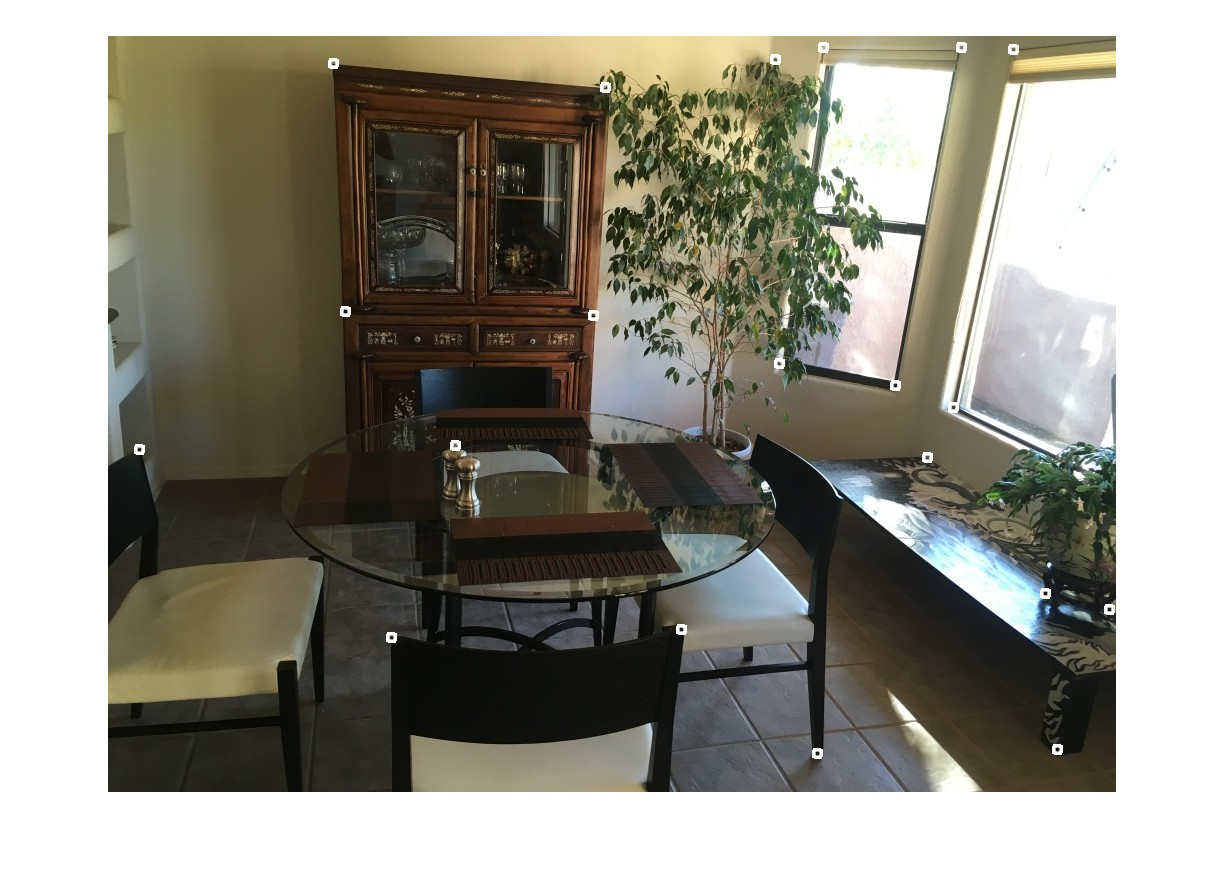
\includegraphics[width=3in]{new_figs/fm1_kp.jpg}}
	\caption{20 keypoints for scene 1}
	\end{subfigure}
	\begin{subfigure}{0.5\textwidth}
    {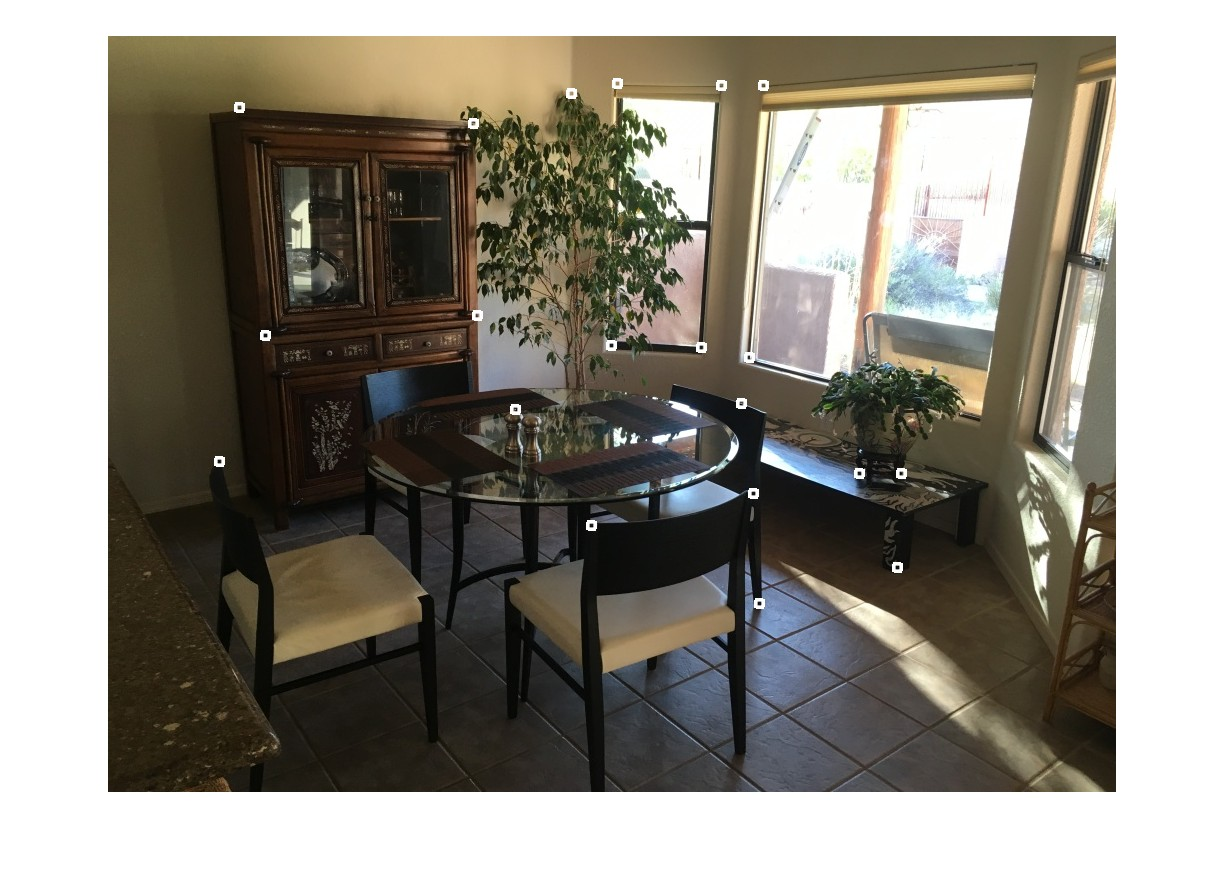
\includegraphics[width=3in]{new_figs/fm2_kp.jpg}
	\caption{20 keypoints for scene 2}
	\end{subfigure}
	\caption{Figure showing matches across two arbitrary views of the same scene. The image points were chosen carefully such that the points occur in both scence.}
\label{fig:fmkeypoints}
\end{figure}


\subsection{} 

Using the fact that $(x')^T F x = 0$ everytime, we can compute the fundamental matrix in the following way. Let:
\begin{equation*}
{\mathbf X'} = 
\begin{bmatrix}
x' \\
y' \\
1
\end{bmatrix},
\quad
{\mathbf X} = 
\begin{bmatrix}
x \\
y \\
1
\end{bmatrix},
\quad
{\mathbf F} = 
\begin{bmatrix}
F_{11} & F_{12} & F_{13}\\
F_{21} & F_{22} & F_{23}\\
F_{31} & F_{32} & F_{33}
\end{bmatrix},
\end{equation*}

Then we have:
\begin{equation*}
\begin{bmatrix}
x' & y' & 1 \\
\end{bmatrix} 
\begin{bmatrix}
F_{11} & F_{12} & F_{13}\\
F_{21} & F_{22} & F_{23}\\
F_{31} & F_{32} & F_{33}
\end{bmatrix}
\begin{bmatrix}
x \\
y \\
1
\end{bmatrix}
= 0
\end{equation*}

\begin{equation*}
\implies
\begin{bmatrix}
x'F_{11} + y'F_{21} + F_{31} & x'F_{12} + y'F_{22} + F_{32} & x'F_{13} + y'F_{23} + F_{33}
\end{bmatrix}
\begin{bmatrix}
x \\
y \\
1
\end{bmatrix}
 = 0
\end{equation*}

Let ${\mathbf F_i}$ be the row vectors of the matrix $F$ for $i = \{1, 2, 3\}$.
\begin{equation*}
\implies
\begin{bmatrix}
\begin{bmatrix}
x' & y' & 1 \\
\end{bmatrix} \cdot {\mathbf F_1}^T

&

\begin{bmatrix}
x' & y' & 1 \\
\end{bmatrix} \cdot {\mathbf F_2}^T

& 

\begin{bmatrix}
x' & y' & 1 \\
\end{bmatrix} \cdot {\mathbf F_3}^T

\end{bmatrix}
\begin{bmatrix}
x \\
y \\
1
\end{bmatrix}
 = 0
\end{equation*}


Therefore, we have:
\begin{equation*}
\begin{bmatrix}
x'x & y'x & x & x'y & y'y & y & x' & y' & 1 
\end{bmatrix} 
\begin{bmatrix}
F_{11} \\
F_{12} \\
F_{13} \\
F_{21} \\
F_{22} \\
F_{23} \\
F_{31} \\
F_{32} \\
F_{33}
\end{bmatrix}
= 0,
\end{equation*}

which we can solve using homogenous least squares method for any number of points ${\mathbf X}$ and corresponding ${\mathbf X'}$. 

\subsection{} 
Using the derivation in Part 5.2, we find $F$ using the 12 (training) coordinates collected in Part 5.1. We tested the computed $F$ on the other $8$ coordinates and yielded an RMS of $0.0249$. 

\subsection{}
Using the given image-pairs and the clicked point-pairs, for this part we used the derived $F$ to draw the epipolar line on both images for each point in the other image. Fig.~\ref{fig:mirrors} shows these lines together with the marked points. On observation, it looks like that the epipolar lines help determine the position of the camera for both scenes! (This question was a lot of fun to tackle.)

\begin{figure}[ht]
\centering
	\begin{subfigure}{0.5\textwidth}
    {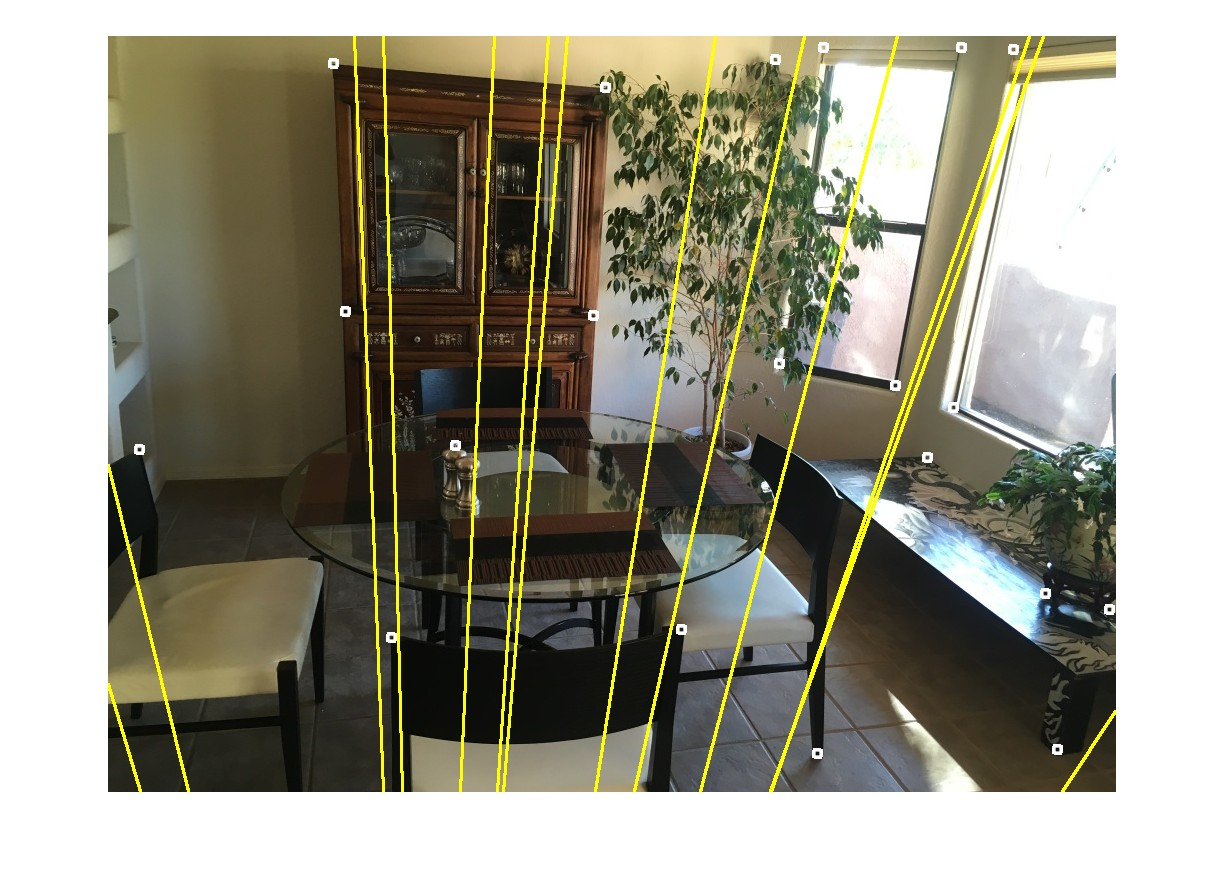
\includegraphics[width=3in]{new_figs/ep1-d1.jpg}}
	\caption{Epipolar lines on scene 1 using points from scene 2}
	\end{subfigure}
	\begin{subfigure}{0.5\textwidth}
    {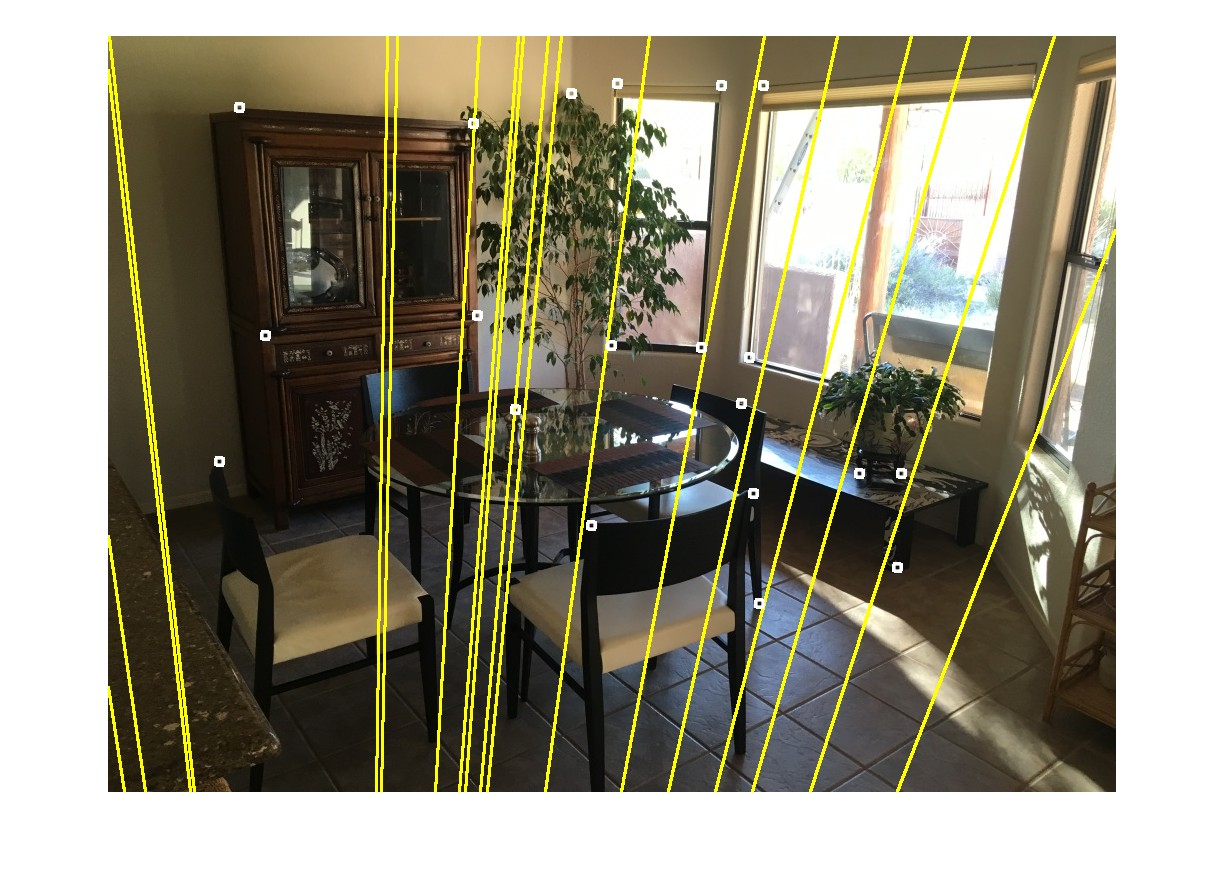
\includegraphics[width=3in]{new_figs/ep2-d1.jpg}
	\caption{Epipolar lines on scene 2 using points from scene 1}
	\end{subfigure}
	\caption{Figure showing epipolar lines on both scences. These were determined by first collecting 20 points by mouse-clicking and then distribution the points into training (of 12 points) and test (of 8 points) sets. Using the training points, we determined the fundamental matrix $F$ using the derivation in 5.2 and used the 8 test points to see how close they are to 0, since $(x')^T F x = 0$ everytime.}
\label{fig:mirrors}
\end{figure}

\section{D2: Image Stitching}
(Will be turned in with HW12)
% \section{Conclusion}
% Conclusion


\end{document}
